\documentclass[a4paper]{article}
\usepackage[utf8]{inputenc}
\usepackage[T1]{fontenc}
\usepackage[spanish]{babel}
\usepackage{listings}
\usepackage{hyperref}
\usepackage{graphicx}
\usepackage{gensymb}
\usepackage{comment}
\usepackage{listings}
\usepackage[official]{eurosym}
\usepackage{color}
\definecolor{lightgray}{rgb}{.9,.9,.9}
\definecolor{darkgray}{rgb}{.4,.4,.4}
\definecolor{purple}{rgb}{0.65, 0.12, 0.82}

\lstdefinelanguage{JavaScript}{
  keywords={typeof, new, true, false, catch, function, return, null, catch, switch, var, if, in, while, do, else, case, break},
  keywordstyle=\color{blue}\bfseries,
  ndkeywords={class, export, boolean, throw, implements, import, this},
  ndkeywordstyle=\color{darkgray}\bfseries,
  identifierstyle=\color{black},
  sensitive=false,
  comment=[l]{//},
  morecomment=[s]{/*}{*/},
  commentstyle=\color{purple}\ttfamily,
  stringstyle=\color{red}\ttfamily,
  morestring=[b]',
  morestring=[b]"
}

\lstset{
   language=JavaScript,
   backgroundcolor=\color{lightgray},
   extendedchars=true,
   basicstyle=\footnotesize\ttfamily,
   showstringspaces=false,
   showspaces=false,
   numbers=left,
   numberstyle=\footnotesize,
   numbersep=9pt,
   tabsize=2,
   breaklines=true,
   showtabs=false,
   captionpos=b
}



\title{PLD: Propuesta del Juego}
\author{Jose Miguel Colella (Y1453965B) y\\José Manuel Gómez González (45920481-S)}


\begin{document}

\maketitle

\section{Propuesta}

\begin{description}
  \item[Título provisional del videojuego] \hfill \\
  Nuestro juego tiene el siguiente título provisional: \textbf{Treasure Hunter}
  \item[Descripción general] \hfill \\
   Se tratará de un juego en 2D de estrategia por turnos. El
escenario es el interior de un complejo secreto (habitaciones, pasillos,
corredores ...). El objetivo consiste en robar un objeto del que se
conocen posibles ubicaciones que el jugador deberá probar para
finalmente huir con el objeto. Un jugador adversario controlado por IA
tendrá el mismo objetivo. Adicionalmente, otra IA controlará varios
agentes encargados de vigilar y atacar a cualquier intruso (el propio
jugador y la otra IA). Como elementos adicionales sobre el escenario
tenemos: interruptores de control, puertas y lasers. Los interruptores
de control abren/cierran (o activan/desactivan) puertas y lasers. Los
lasers a la altura de la cintura solo afectan a los jugadores (usuario e
IA) quitandoles puntos de vida. Las puertas afectan a todos al bloquear
el paso. La dificultad vendrá dada por la IA y por el propio mapa.
Otro punto interesante aunque complementario sería la
posibilidad de generar mapas de manera automática.
  \item[Género] \hfill \\
  \href{http://en.wikipedia.org/wiki/Video_game_genre#Turn-based_strategy}{Turn Based Strategy Game}
  \item[Audiencia]
  Cualquier tipo de persona es capaz de juegar el juego aunque tiene una tematica de puede
  ser influencial en jovenes

  \item[3 videojuegos del mismo segmeto]
    \begin{enumerate}
      \item
      \begin{description}
        \item[Título] \hfill \\
        Rome Total War 2
        \item[Compañia] \hfill \\
        Creative Assembly \\Sega
        \item[Plataforma] \hfill \\
        PC (Microsoft Windows, Linux)
        \item[Comercialización] \hfill \\
        DVD, Descarga por Steam 54,99 \euro{}
        \item[Página web] \hfill \\
        \hyperlink{http://www.totalwar.com/en_us/rome2/}{Rome Total War 2}
        \item[Capturas de pantalla] \hfill \\
        \begin{figure}[ht!]
        \centering
        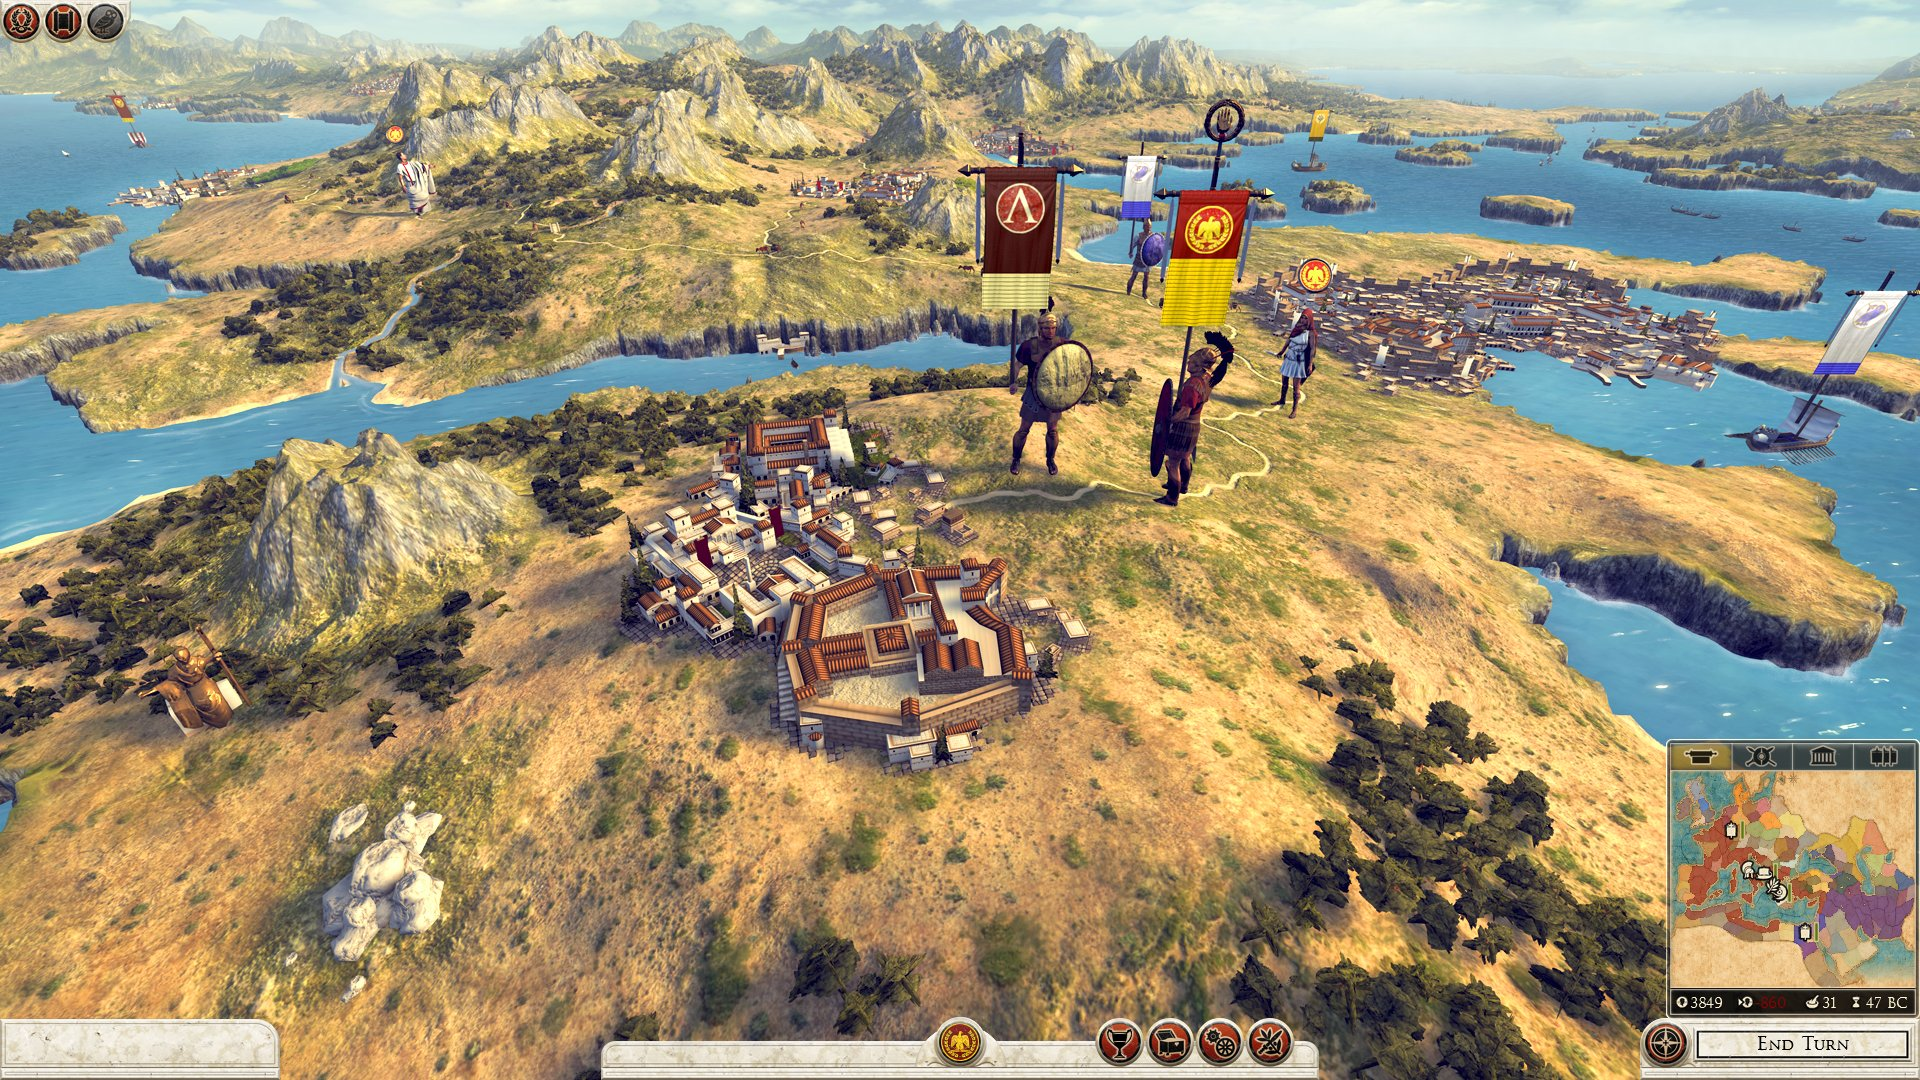
\includegraphics[width=90mm]{./Total-War-Rome-2-11.jpg}
        \caption{Campaña Turn Based Strategy}
        \label{overflow}
        \end{figure}
        \begin{figure}[ht!]
        \centering
        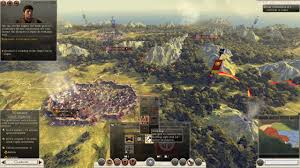
\includegraphics[width=90mm]{./images.jpeg}
        \caption{El juegador controla ciudades y pelea por establecer su dominio}
        \label{overflow2}
        \end{figure}
        \item[3 características destacadas] \hfill \\
          \begin{enumerate}
            \item Las gráficas del juego son extraordinarias
            \item La inteligencia artificial es robusta
            \item Basado en hechos reales
          \end{enumerate}
        \item[3 limitaciones observadas] \hfill \\
          \begin{enumerate}
            \item Cuando se juega en modo difícil la inteligencia artificial toma mucho tiempo
            en hacer una decisión
            \item Unas veces IA no toma decisiones que beneficia el grupo que representa
            \item Tienes que tener capacidades gráficas muy buenas para tener muy buenas FPS (Frames per seconds).
          \end{enumerate}
      \end{description}
      \item
      \begin{description}
        \item[Título] \hfill \\
        Sid Meier's Civilization
        \item[Compañia] \hfill \\
        Firaxis Game\\ 2K Games \& Aspyr
        \item[Plataforma] \hfill \\
        PC (Microsoft Windows), OSX, \href{http://en.wikipedia.org/wiki/OnLive}{OnLive}
        \item[Comercialización] \hfill \\
        DVD, Descarga en Steam 29.99 \euro{}, Cloud Computing
        \item[Página web] \hfill \\
        \hyperlink{http://www.civilization5.com/}{Rome Total War 2}
        \item[Capturas de pantalla] \hfill \\
        \begin{figure}[ht!]
        \centering
        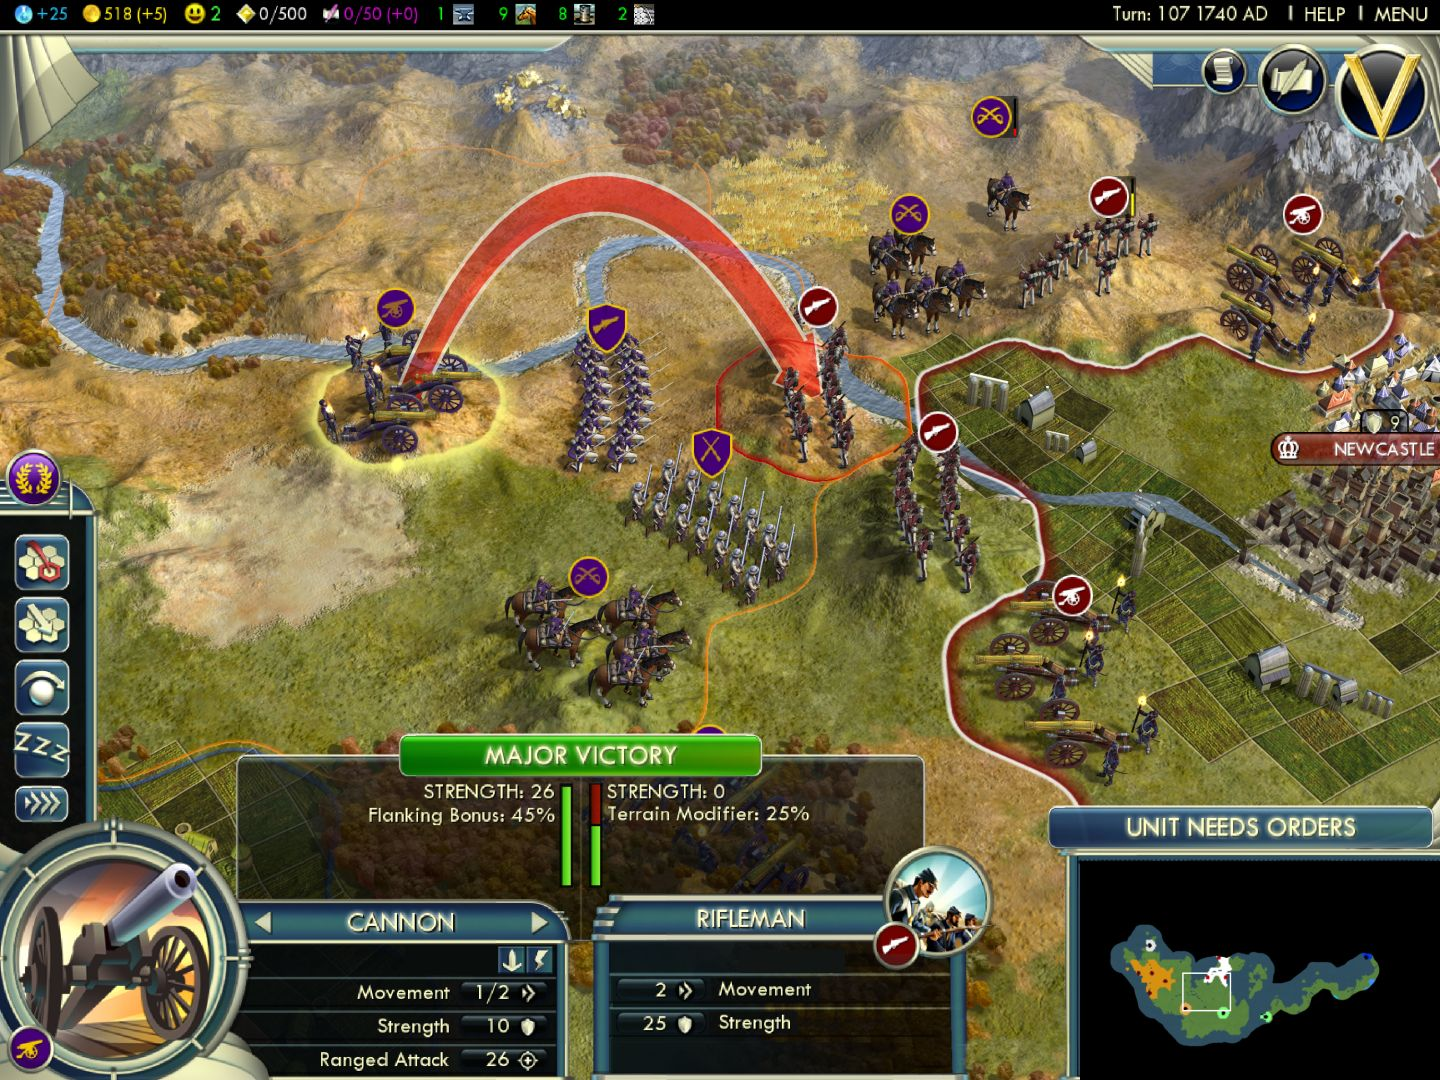
\includegraphics[width=90mm]{./civilization.jpg}
        \caption{Campaña Turn Based Strategy}
        \label{overflow}
        \end{figure}
        \item[3 características destacadas] \hfill \\
          \begin{enumerate}
            \item
            \item
            \item
          \end{enumerate}
        \item[3 limitaciones observadas] \hfill \\
          \begin{enumerate}
            \item
            \item
            \item
          \end{enumerate}
      \end{description}

    \end{enumerate}

\end{description}

\end{document}

